\documentclass{article}
\usepackage[top=1cm,left=1cm,right=1cm]{geometry}
\usepackage[T1]{fontenc}
\usepackage{setspace}
\usepackage[normalem]{ulem} %underline with proper breaking
\usepackage{microtype} %typographical refinements

\usepackage{mathtools,mathrsfs,amssymb,amsthm}
\everymath{\displaystyle}
\newcommand{\norm}[1]{\ensuremath{\left\|#1\right\|}}
\renewcommand{\vec}{\mathbf}

\usepackage{arydshln} %lines in arrays
\usepackage[dvipsnames]{xcolor}
\usepackage{tikz}
\usetikzlibrary[arrows,patterns,decorations.markings]

\begin{document}
\begin{center}
	{\LARGE \textbf{Formal Project Proposal}}

	\vspace{5mm}
	{\Large Kevin Wang}
\end{center}

\subsection*{Program Description}

The program is written in Processing and simulates the motion of particles acting under gravity. The concepts of Newton's law of gravitation, Newton's second law, and conservation of linear momentum are demonstrated, with the last one through particle collisions.

The program involves a canvas where the particles are simulated. Alongside the simulation is a panel that displays some properties of the system. As for user interaction, the user is able to create new particles and adjust the values of the gravitational constant, masses of the particles, and elasticity of the particles.

\subsection*{Underlying Math}

Newton's law of gravitation in vector form is
\[\vec{F}_{21}=-G\frac{m_1m_2}{\norm{\vec{r}_2-\vec{r}_1}^2}\frac{\vec{r}_2-\vec{r}_1}{\norm{\vec{r}_2-\vec{r}_1}}\]
where $\vec{F}_{21}$ is the force applied on particle 2 exerted by particle 1, $G$ is the gravitational constant, $m_1,m_2$ are the masses of the particles, and $\vec{r}$ is a position vector.

The form of Newton's second law used in the program is
\[\sum\vec{F}=m\vec{a}.\]
The position of the particles will be solved using numerical methods.

The equations used for calculating the results of particle collisions are
\[
\begin{cases}
	\vec{v}_a=\frac{C_Rm_b(\vec{u}_b-\vec{u}_a)+m_a\vec{u}_a+m_b\vec{u}_b}{m_a+m_b}\\
	\vec{v}_b=\frac{C_Rm_a(\vec{u}_a-\vec{u}_b)+m_a\vec{u}_a+m_b\vec{u}_b}{m_a+m_b}
\end{cases}
\]
where $\vec{u}_a,\vec{u}_b$ are the initial velocities of the particles, $\vec{v}_a,\vec{v}_b$ are the final velocities of the particles, $m_a,m_b$ are the masses of the particles, and $C_R$ is the coefficient of restitution. A $C_R$ of 0 indicates a perfectly inelastic collision and a $C_R$ of 1 indicates an elastic collision.

The center of mass calculation is done by
\[\vec{R}=\frac{1}{M}\sum_im_i\vec{r}_i.\]

\subsection*{Assumptions and Restrictions in the Simulation}

\begin{itemize}
	\item The particles are treated as being massive enough to gravitationally attract one another.
	\item The maximum number of particles allowed is six particles.
	\item The masses of the particles is limited to a certain range.
	\item The gravitational constant is limited to a certain range.
	\item All particles have the same mass and elasticity.
	\item All particles are of the same size.
	\item The particles are treated as point masses in collisions (i.e, there is no spin).
\end{itemize}

\subsection*{Game Controls}

Users will use the keyboard and mouse to modify simulation variables and create particles.
\begin{itemize}
	\item \textbf{Up} increase the elasticity of the particles
	\item \textbf{Down} decrease the elasticity of the particles
	\item \textbf{A} increase the mass of the particles
	\item \textbf{D} decrease the mass of the particles
	\item \textbf{W} increase the gravitational field strength
	\item \textbf{S} decrease the gravitational field strength
	\item To create particles, click in the canvas and direct the mouse in the direction of the velocity. The magnitude of the arrow corresponds to the magnitude of the velocity.
\end{itemize}

\subsection*{Visual Elements}

\begin{itemize}
	\item Particles have different colors
	\item Location of the center of mass for the system
	\item Kinetic energy of the system of particles
	\item Values of the gravitational constant, elasticity, and mass
\end{itemize}
\begin{figure}[h]
	\centering
	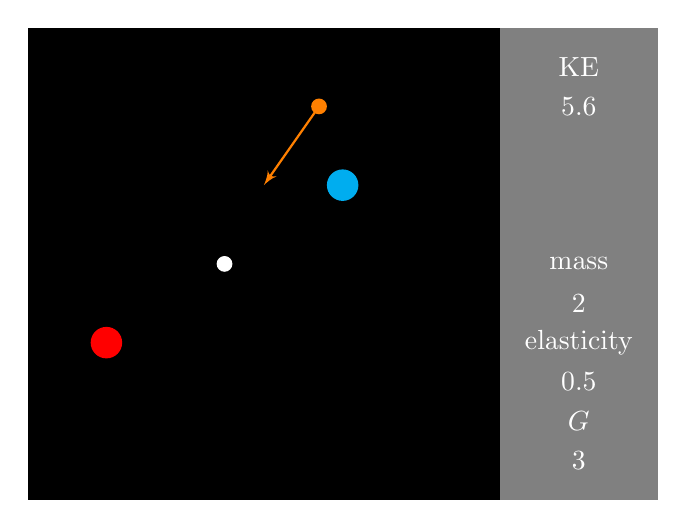
\begin{tikzpicture}[>=latex',thick]
		\fill (0,0) rectangle (6,6);
		\fill[gray] (6,0) rectangle (8,6);
		\fill[red] (1,2) circle (2mm);
		\fill[cyan] (4,4) circle (2mm);
		\fill[white] (2.5,3) circle (1mm);
		\fill[orange] (3.7,5) circle (1mm);
		\draw[->,orange] (3.7,5) -- (3,4);
		\draw (7,5.5) node[white] {KE};
		\draw (7,5) node[white] {5.6};
		\draw (7,3) node[white] {mass};
		\draw (7,2.5) node[white] {2};
		\draw (7,2) node[white] {elasticity};
		\draw (7,1.5) node[white] {0.5};
		\draw (7,1) node[white] {$G$};
		\draw (7,0.5) node[white] {3};
	\end{tikzpicture}
	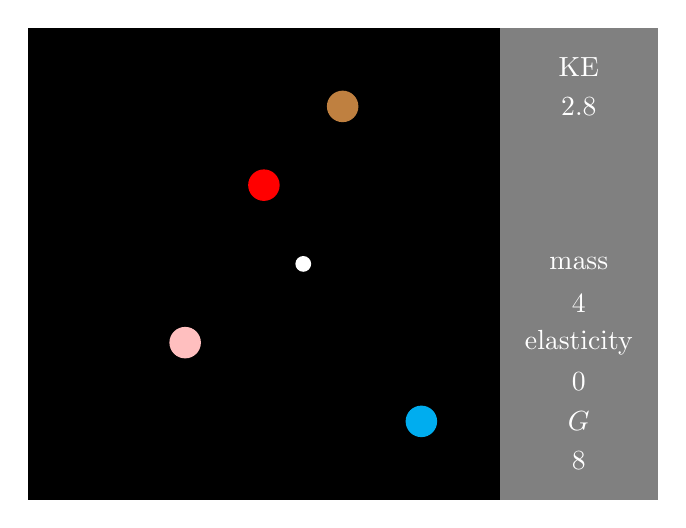
\begin{tikzpicture}[>=latex',thick]
		\fill (0,0) rectangle (6,6);
		\fill[gray] (6,0) rectangle (8,6);
		\fill[red] (3,4) circle (2mm);
		\fill[cyan] (5,1) circle (2mm);
		\fill[pink] (2,2) circle (2mm);
		\fill[brown] (4,5) circle (2mm);
		\fill[white] (3.5,3) circle (1mm);
		\draw (7,5.5) node[white] {KE};
		\draw (7,5) node[white] {2.8};
		\draw (7,3) node[white] {mass};
		\draw (7,2.5) node[white] {4};
		\draw (7,2) node[white] {elasticity};
		\draw (7,1.5) node[white] {0};
		\draw (7,1) node[white] {$G$};
		\draw (7,0.5) node[white] {8};
	\end{tikzpicture}
\end{figure}

\subsection*{Additional Stuff if Time Allows}

\begin{itemize}
	\item show forces acting on each individual particle
	\item make the particles charged
	\item remove some of the assumptions or restrictions
\end{itemize}

\subsection*{Bugs}

\begin{itemize}
	\item numerical approximations are not exact and strange fluctuations can occur due to floating point calculation errors building up
	\item try out superelastic collisions (coefficient greater than 1): warning: particles gain kinetic energy after collision so use at your own risk
	\item turning on container can result in some unpredictable behavior near the boundaries
\end{itemize}


\end{document}
